\section{Zielsetzung}
Im Versuch wird die Reichweite von Alphastrahlung in Luft ermittelt, sowie der statistische Zerfall analysiert.

\section{Theorie}
Die Entstehung von $\alpha$-Strahlung ist quantenmechanisch erklärbar. Die Kernkräfte und die Abstoßungskräfte der Protonen bilden einen unendlich
hohen Potentialwall. Klassisch ist eine Überwindung dessen nicht erklärbar. Quantenmechanisch besteht jedoch eine Tunnelwahrscheinlichkeit, die
das Überwinden des unendlich hohen Potentialwalls und somit die Entstehung von $\alpha$-Strahlung erklärt.
Beim Durchlaufen von Materie verliert $\alpha$-Strahlung ihre Energie. Dies ist durch drei verschiedene Prozesse zu erklären.
Zum einen durch die sogenannte Rutherford-Streuung, wobei es zu elastischen Stößen zwischen den $\alpha$-Teilchen und den Materieteilchen
kommt, welche für den Energieverlust und somit für den Versuch jedoch nur eine untergeordnete Rolle spielt.
Des weiteren ist ein Energieverlust durch Ionisationsprozesse und Anregung oder Dissoziation von Molekülen zu erklären.
Zu erwähnen ist, dass der Energieverlust der $\alpha$-Strahlung bei kleineren Geschwindigkeiten größer wird, was durch die längere
Zeit zu erklären ist, die die Teilchen zur Wechselwirkung miteinander haben. Außerdem ist der Energieverlust abhängig von der Energie der
$\alpha$-Teilchen selbst, sowie der Dichte des Materials mit dem die Strahlung wechselwirkt.
Die Bethe-Bloch-Gleichung beschreibt den Energieverlust von Teilchen, die eine hinreichend große Anfangsenergie besitzen. Sie verliert ihre
Gültigkeit für $\alpha$-Teilchen mit geringer Energie, weil dann Ladungsaustauschprozesse stattfinden.
\FloatBarrier
\begin{align*}
  - ~\frac{dE_\alpha}{dx} = \frac{z^2~e^4}{4\pi\epsilon_0 m_e}~\frac{n ~ Z}{v^2}~ln\left(\frac{2 m_e v^2}{I}\right) .
\end{align*}
\FloatBarrier
In der Bethe-Bloch-Gleichung beschreibt $z$ die Ladung, $v$ die Geschwindigkeit der $\alpha$-Strahlung, $n$ die Teilchendichte, $Z$ steht für die
Ordnungszahl und $I$ für die Ionisationsenergie des Targetgases.
Die Reichweite von $\alpha$-Strahlung lässt sich dann mittels Integration berechnen:
\FloatBarrier
\begin{align*}
  \int_{0}^{E_{\alpha}} \frac{dE_\alpha}{-dE_\alpha ~ / dx}
\end{align*}
\FloatBarrier
Die mittlere Reichweite $R_m$ von Teilchen mit niedrigerer Energie, bei denen es vermehrt zu Ladungsaustauschprozessen kommt, kann mittels
empirischer gewonnener Kurven bestimmt werden.
Gleichung \ref{eq3} beschreibt die mittlere Reichweite für $\alpha$-Teilchen, die eine Energie unter $\SI{2,5}{\mega \eV}$ besitzen.
Die mittlere Reichweite beschreibt die Distanz, in der noch die Hälfte aller emittierten $\alpha$-Teilchen ankommen.
\FloatBarrier
\begin{align*}
  \label{eq3}
  R_m = 3,1 \cdot E_{\alpha}^{3/2}
\end{align*}
\FloatBarrier
Da die Reichweite von $\alpha$-Strahlung in Gasen druckabhängig ist, gilt zur Ermittlung der Reichweite folgender Zusammenhang:
\begin{align*}
  x = x_0 \frac{p}{p_0}
\end{align*}
Hierbei beschreibt $x_0$ den fixen Abstand zwischen Detektor und Quelle, und $p_0$ den Normaldruck von $\SI{1013}{\bar}$.

\section{Durchführung}
Zur Durchführung des Versuchs wird eine $\alpha$-Strahlungsquelle, ein Detektor, eine Vakuumpumpe zur Evakuierung des Glaszylinders, in dem
sich Quelle und Detektor befinden, ein Vorverstärker, ein Vielkanalanalysator, sowie ein PC, der die vom Detektor gemessenen und vom
Vielkanalanalysator analysierten, Daten aufnimmt, benötigt. Der Versuchsaufbau ist in Abbildung \ref{abb1} zu sehen.
Der Abstand der Quelle ist variabel einzustellen und an einer Skala, die außen auf dem Glaszylinder aufgezeichnet ist, abzulesen.
Der Detektor ist ein Halbleiter-Sperrschichtzähler, welcher den Vorteil besitzt, dass er dazu in der Lage ist Strahlung mit niedrigerer Energie
zu detektieren. Dies geschieht, indem einfallende Ionen in der Sperrschicht des Halbleiters ein Elektron-Loch-Paar erzeugen, welches zu
einem Strompuls im Halbleiter führen, welcher gemessen werden kann. Die erzeugten Pulse werden von dem Vorverstärker verstärkt, vom
Vielkanalanalysator analysiert und an das PC-Programm "Multichannel Analyzer" weitergegeben. Im Programm werden die Pulshöhen, die der Energie
der $\alpha$-Strahlung entsprechen, als Histogramm dargestellt.
\FloatBarrier
\begin{figure}
  \centering
  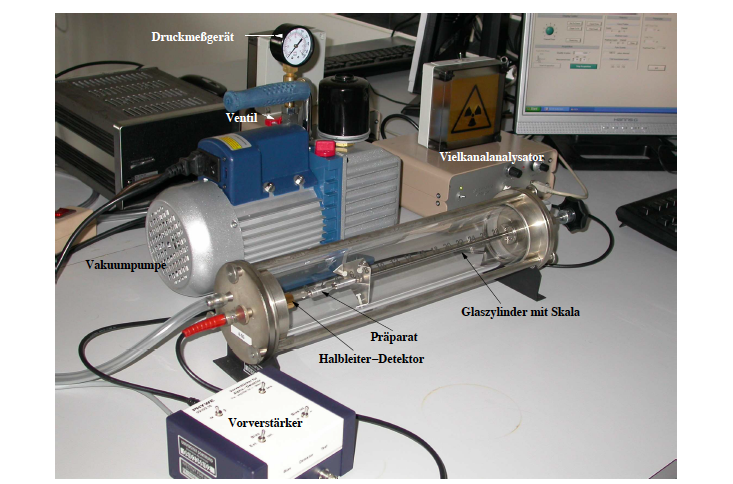
\includegraphics[scale=0.6]{Aufbau.PNG}
  \caption{Versuchsaufbau \cite{Q1}.}
  \label{abb1}
\end{figure}
\FloatBarrier
\noindent Im ersten Teil des Versuchs muss zu Beginn der Glaszylinder evakuiert werden. Die Messdauer eines jeden Schrittes beträgt zwei Minuten.
Nach zwei Minuten Messdauer werden dann die gemessenen Counts insgesamt, die Counts, die sich um das Maximum herum befinden, sowie die
Lage des Maximums notiert. Es wird davon ausgegangen, dass die detektierte $\alpha$-Strahlung bei $\SI{0}{\milli \bar}$ eine Energie
von $\SI{4}{\mega \eV}$ besitzt. Aus der Anzahl der Counts im Maximum lässt sich mittels Dreisatz die Energie für höhere Drücke
berechnen. Der Druck wird schrittweise um $\SI{50}{\milli \bar}$ erhöht und die drei oben erwähnten Werte werden jeweils nach zwei Minuten Messzeit
notiert. Der Druck kann bis $\SI{1000}{\milli \bar}$ erhöht werden. Es ist daher wichtig, dass im Vorfeld klargestellt wurde, dass die Apparatur
so eingestellt ist, dass bei diesem maximalen Druck nur noch sehr wenige bis gar keine Counts insegsamt mehr detektiert werden.
Am Versuchstag wurde diese Überprüfung bereits im Vorfeld, jedoch nicht von uns durchgeführt.
Die oben beschriebene Messung wird einmal bei einem Abstand zwischen Quelle und Detektor von $\SI{2}{\cm}$ und ein weiteres Mal für einen Abstand
von $\SI{2,5}{\cm}$ durchgeführt.

\noindent Zur Ermittlung des statistischen Zerfalls werden im evakuierten Glaszylinder für 100 Messungen bei einem Abstand von $\SI{2}{\cm}$
über $\SI{10}{\second}$ die Gesamtcounts gemessen und notiert. Die Zerfallsraten werden sodann in einem Histogramm aufgetragen und es werden
Mittelwert und Varianz der Zählraten bestimmt. Anschließend werden die Ergebnisse mit der Poisson- und der Gaußverteilung verglichen.

\section{Auswertung}
\subsection{Bestimmung der Reichweite von Alpha-Strahlung}
Die Messwerte zur Bestimmung der Reichweite von Alpha-Strahlung bei $x_0=\SI{2}{\centi\meter}$ sind in Tabelle \ref{tab:1} aufgelistet, wobei $x_0$
den Abstand zwischen der Quelle und dem Detektor beschreibt.
Zur Bestimmung der Abhängigkeit der Energie $E$ vom Druck $p$, muss zunächst die Energie berechnet werden. Hierzu wird von einer linearen
Energieskala ausgegangen, wobei die Alpha-Teilchen bei dem Druck $p=\SI{0}{\bar}$ eine Energie von $\SI{4}{\mega\eV}$ besitzen. Diese Energien können
mittels Dreisatz für alle anderen Messungen berechnet werden:
\begin{equation*}
  E(p)= \frac{C(p)}{C(p=0)} \cdot \SI{4}{\mega\eV}
\end{equation*}
Die Enerige $E(p)$  wird in Abhängigkeit des Drucks $p$ ist in Abbildung \ref{abb:1} aufgetragen.
\begin{figure}
  \centering
  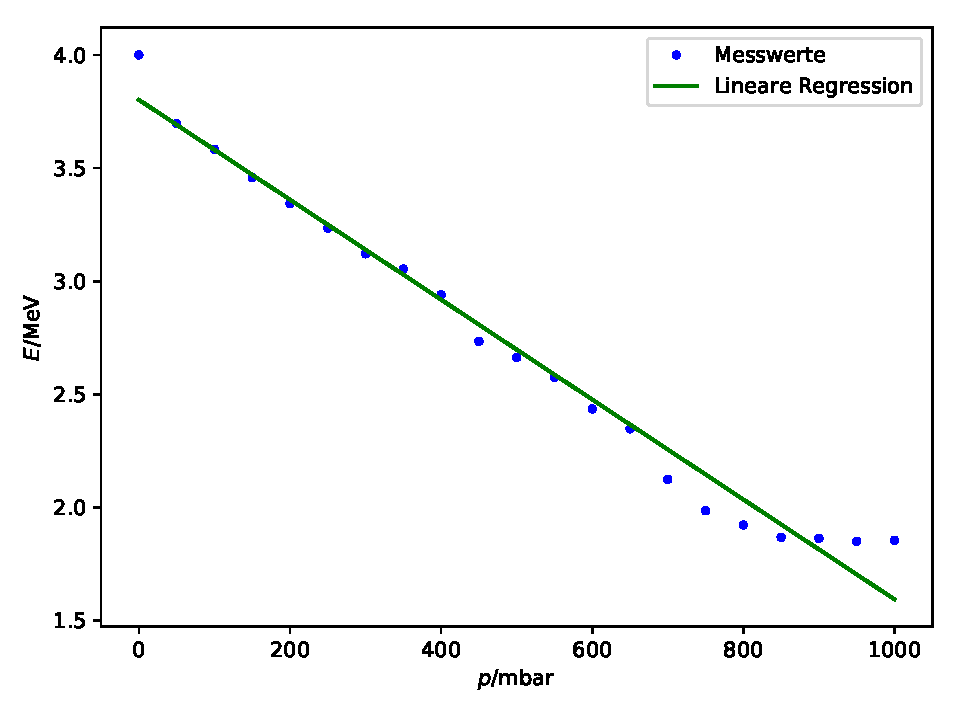
\includegraphics[scale=0.6]{Messung1b.pdf}
  \caption{Enerige $E$ in Abhängigkeit des Drucks $p$.}
  \label{abb:1}
\end{figure}
Mittels einer linearen Regression der Form $E(p)=a\,p+b$ kann die Funktion für $E(p)$ ermittelt werden:
\begin{align*}
  a&= \SI{-2,21(7)}{\mega\eV\per\milli\bar} \\
  b&= \SI{3,80(4)}{\mega\eV}\\
  E(p)&= -2,21 \cdot p +3,8
\end{align*}
wobei $E$ in \si{\mega\eV} und $p$ in \si{bar}.


Des weiteren soll die mittlere Reichweite der Alpha Teilchen bestimmt werden, die Messwerte zu diesem Versuchsteil sind in Tabelle \ref{tab:1} und
\ref{tab:2} aufgelistet. Zur Bestimmung der mittleren Reichweite wird in Abbildung \ref{abb:2} die Rate $R$ der "Pulses Detected", also
$R=\frac{N_{\symup{gesamt}}}{\symup\Delta t}$, gegen die effektive Länge aufgetragen, hierbei ist $\symup\Delta t = \SI{120}{\second}$ das Messintervall
und $N_{\symup{gesamt}}$ die gemessenen Impulse in dem Zeitintervall.
Die effektive Länge $x$ lässt sich aus dem gemessenen Druck $p$ berechnen mit Hilfe der Formel
\begin{equation*}
  x = x_0 \cdot \frac{p}{p_0}
\end{equation*}
wobei $x_0$ den Abstand zwischen der Quelle und dem Detektor und $p_0=\SI{1013,25}{\milli\bar}$ den Atmosphärendruck beschreibt.
Die Messung für $x_0=\SI{2}{\centi\meter}$ ist in Abbildung \ref{abb:2} zu sehen und die Messung für $x_0={2,5}{\centi\meter}$ in Abbildung \ref{abb:3}.

Zur Bestimmung der mittleren Reichweite der Alpha-Teilchen wird eine lineare Regression ab dem Abfall der Messwerte druchgeführt. Die mittlere Reichweite ist
als die Reichweite definiert, bei der nurnoch die Hälfte der "Impulse detected" erfasst werden. Damit kann nun die mittlere Reichweite berechnet werden.
Die lineare Regression der Form $N_{\symup{gesamt}}(x)=m\cdot x+b$ liefert die Werte für beide Messungen
\begin{align*}
  m_1 &= \SI{-750(70)}{\per\second\per\centi\meter}\\
  b_1 &= \SI{1,47(11)}{\per\milli\second}\\
  m_2 &= \SI{,610(50)}{\per\second\per\centi\meter}\\
  b_2 &= \SI{1,31(9)}{\per\milli\second}
\end{align*}
Daraus folgt für die mittleren Reichweiten $\overline{x}$:
\begin{align*}
  \frac{R_1}{2} &= \SI{328,95}{\per\second}\\
  \overline{x}_1 &= \SI{15,3}{\milli\meter} \\
  \frac{R_2}{2} &= \SI{262,54}{\per\second}\\
  \overline{x}_2 &= \SI{17,3}{\milli\meter} \\
\end{align*}
Aus den mittleren Reichweiten lassen sich die Energien mittels der Formel
\begin{equation*}
  E = \left(\frac{\overline{x}}{3.1} \right)^{\frac{2}{3}}
\end{equation*}
berechenen, wobei $\overline{x}$ in \si{\milli\meter} und $E$ in \si{\mega\eV} angegeben wird. Daraus folgt für die Energien
\begin{align*}
  E_1= \SI{2,899}{\mega\eV} \\
  E_2= \SI{3,146}{\mega\eV}
\end{align*}
Weiterführend soll außerdem noch der Energieverlust $-\frac{\symup d E}{\symup d x}$ für die erste Messung ($x_0=\SI{2}{\centi\meter}$) bestimmt werden.
Hierzu wird die Energie $E$ in Abhängigkeit der effektiven Reichweite $x$ gegeneinander aufgetragen (siehe Abbildung \ref{abb:5}). Bei den Messwerten wird
eine lineare Regression der Form $E(x)=ex+E_0$ durchgeführt. Diese liefert die Werte:
\begin{align*}
  e&=\SI{-1,12(4)}{\mega\eV\per\centi\meter} \\
  E_0 &=\SI{3,80(4)}{\mega\eV}
\end{align*}
Der Energieverlust lässt sich somit aus der Steigung ablesen:
\begin{equation*}
  -\frac{\symup d E}{\symup d x} = -e = \SI{1,12(4)}{\mega\eV\per\centi\meter}
\end{equation*}

\subsection{Statistik}
Zur Überprüfung der Statistik werden 100 Messwerte in einer Zeitdauer von $\symup\Delta t= \SI{10}{\second}$ aufgenommen, diese Messwerte sind in
Tabelle \ref{tab:3} aufgelsitet.
Zur Berechnung des Mittelwertes und die Standardabweichung wird wie folgt berechnet:
\begin{align*}
  \overline{N} &= \frac{\sum\limits_{i=1}^{100} N_i}{100} = 5156,14 \\
  \sigma_N &= \sqrt{\frac{\sum\limits_{i=1}^{100}(N_i-\overline{N})}{100}} = 206,16
\end{align*}
Das Histogramm der Messwerte und der Verteilungen (Poisson- und Normalverteilung) sind in Abbildung \ref{abb:4} dargestellt.


\begin{figure}[h!]
  \centering
  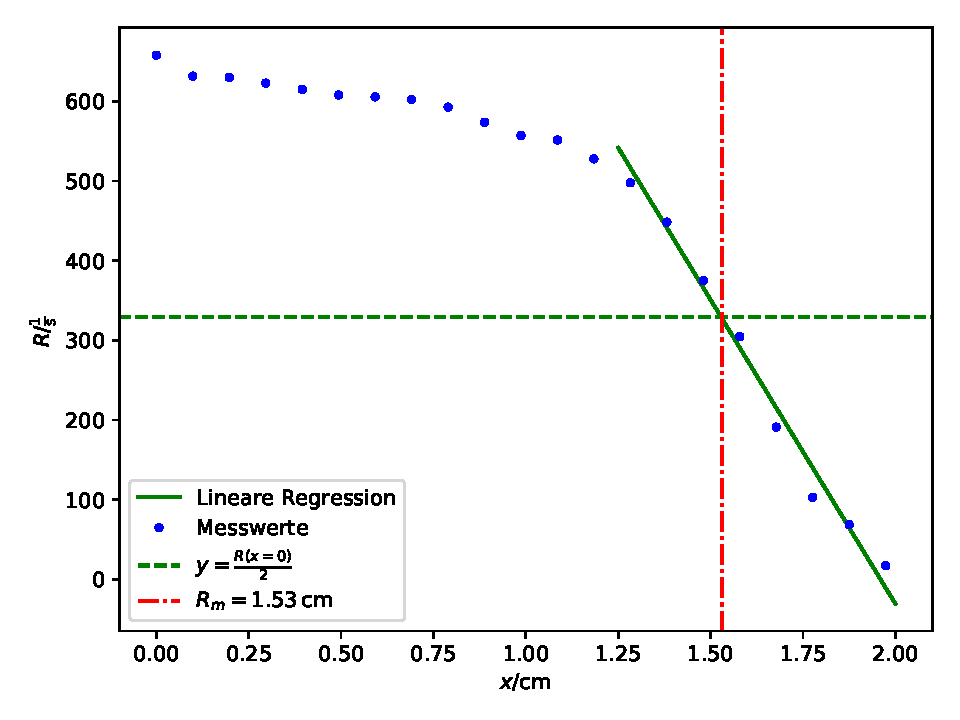
\includegraphics[scale=0.6]{Messung1a.pdf}
  \caption{Rate $R$ in Abhängikeit der effektiven Reichweite $x$ für $x_0=\SI{2}{\centi\meter}$.}
  \label{abb:2}
\end{figure}
\begin{figure}[h!]
  \centering
  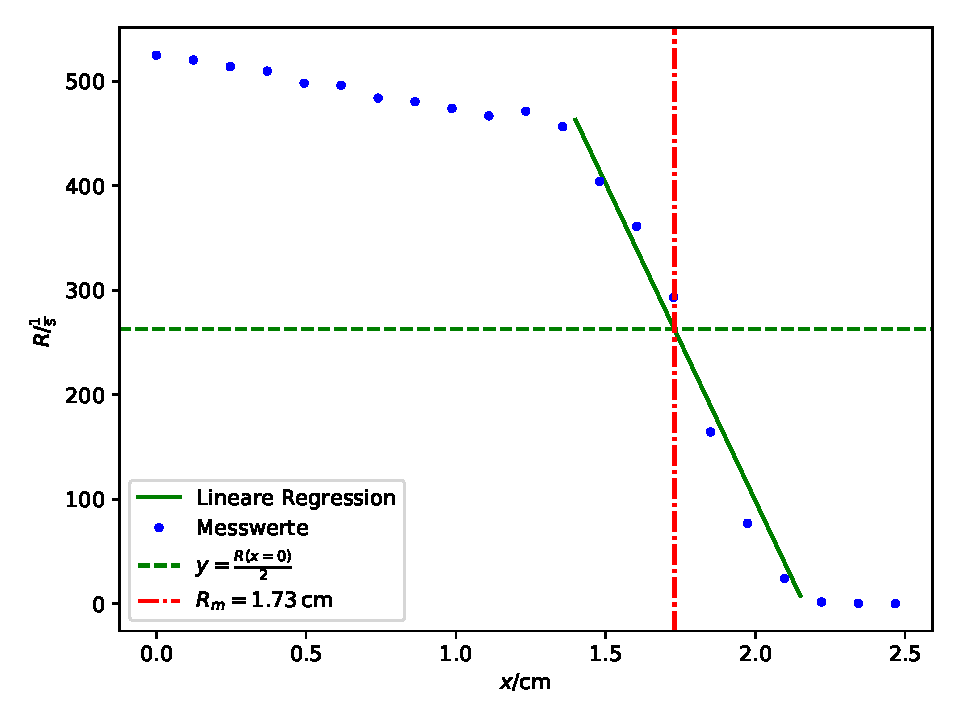
\includegraphics[scale=0.6]{Messung2a.pdf}
  \caption{Rate $R$ in Abhängikeit der effektiven Reichweite $x$ für $x_0=\SI{2,5}{\centi\meter}$.}
  \label{abb:3}
\end{figure}
\begin{table}[h!]
  \centering
  \caption{Messwerte: Reichweite der Alpha-Strahlung bei $x_0=2 \, \mathrm{cm}$}
  \label{tab:1}
  \begin{tabular}{c c c c c}
    \toprule
    Druck & Counts & Channel & Pulses detected & Enerige \\
    $p$ / \si{\milli\bar} & $N$ & $C$ & $N_{\symup{gesamt}}$ & $E$ / \si{\mega\eV} \\
    \midrule
    0 & 212 & 951 & 78949 & 4,00 \\
    50 & 219 & 879 & 75793 & 3,70 \\
    100 & 223 & 852 & 75596 & 3,58 \\
    150 & 227 & 822 & 74744 & 3,46 \\
    200 & 239 & 795 & 73799 & 3,34 \\
    250 & 246 & 769 & 72949 & 3,23 \\
    300 & 263 & 742 & 72668 & 3,12 \\
    350 & 281 & 726 & 72257 & 3,05 \\
    400 & 272 & 699 & 71129 & 2,94 \\
    450 & 280 & 650 & 68861 & 2,73 \\
    500 & 297 & 633 & 66846 & 2,66 \\
    550 & 309 & 612 & 66164 & 2,57 \\
    600 & 314 & 579 & 63336 & 2,44 \\
    650 & 331 & 558 & 59725 & 2,35 \\
    700 & 329 & 505 & 53819 & 2,12 \\
    750 & 334 & 472 & 44985 & 1,99 \\
    800 & 344 & 457 & 36568 & 1,92 \\
    850 & 299 & 444 & 22941 & 1,87 \\
    900 & 195 & 443 & 12352 & 1,86 \\
    950 & 189 & 440 & 8248 & 1,85 \\
    1000 & 55 & 441 & 2060 & 1,85 \\
    \bottomrule
  \end{tabular}
\end{table}

\begin{table}[h!]
  \centering
  \caption{Messwerte: Reichweite der Alpha-Strahlung bei $x_0=2,5 \, \mathrm{cm}$}
  \label{tab:2}
  \begin{tabular}{c c c c}
    \toprule
    Druck & Counts & Channel & Pulses detected \\
    $p$ / \si{\milli\bar} & $N$ & $C$ & $N_{\symup{gesamt}}$ \\
    \midrule
    0 & 174 & 904 & 63009 \\
    50 & 184 & 881 & 62457 \\
    100 & 182 & 826 & 61698 \\
    150 & 199 & 804 & 61184 \\
    200 & 205 & 774 & 59786 \\
    250 & 219 & 746 & 59545 \\
    300 & 212 & 719 & 58084 \\
    350 & 233 & 689 & 57667 \\
    400 & 235 & 654 & 56901 \\
    450 & 245 & 633 & 56036 \\
    500 & 251 & 623 & 56577 \\
    550 & 240 & 594 & 54787 \\
    600 & 257 & 543 & 48507 \\
    650 & 271 & 508 & 43352 \\
    700 & 322 & 451 & 35190 \\
    750 & 262 & 443 & 19731 \\
    800 & 176 & 440 & 9231 \\
    850 & 73 & 440 & 2882 \\
    900 & 7 & 447 & 191 \\
    950 & 2 & 433 & 33 \\
    1000 & 0 & 0 & 0 \\
    \bottomrule
  \end{tabular}
\end{table}
\begin{figure}
  \centering
  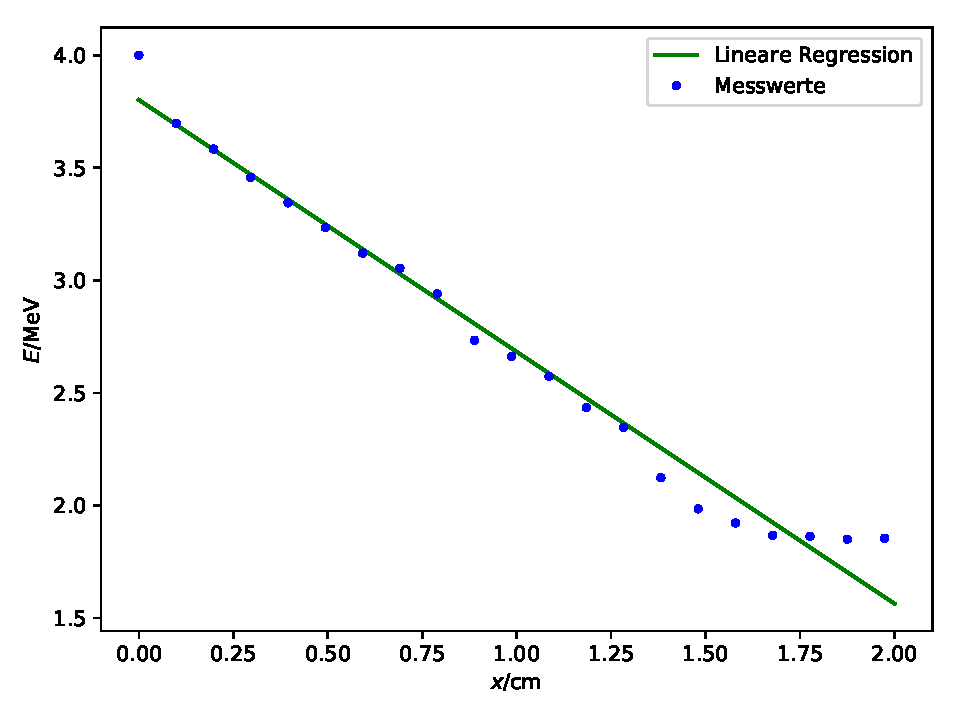
\includegraphics[scale=0.6]{Messung1c.pdf}
  \caption{Berechnung des Energieverlustet.}
  \label{abb:5}
\end{figure}


\begin{table}
  \centering
  \caption{Statistik.}
  \label{tab:3}
  \begin{tabular}{c c|c c|c c|c c}
    \toprule
    Messung & Counts & Messung & Counts & Messung & Counts & Messung & Counts \\
    \midrule
    1 & 5131 & 26 & 5286 & 51 & 5304 & 76 & 5109 \\
    2 & 5555 & 27 & 5440 & 52 & 4875 & 77 & 5117 \\
    3 & 5100 & 28 & 5280 & 53 & 4990 & 78 & 5144 \\
    4 & 5597 & 29 & 5087 & 54 & 4743 & 79 & 4876 \\
    5 & 5502 & 30 & 5227 & 55 & 5136 & 80 & 5214 \\
    6 & 5308 & 31 & 5547 & 56 & 5336 & 81 & 5032 \\
    7 & 5041 & 32 & 5368 & 57 & 5119 & 82 & 5265 \\
    8 & 4854 & 33 & 5182 & 58 & 4966 & 83 & 5115 \\
    9 & 5280 & 34 & 4863 & 59 & 4807 & 84 & 5269 \\
    10 & 5274 & 35 & 5258 & 60 & 5176 & 85 & 4960 \\
    11 & 5156 & 36 & 5523 & 61 & 4855 & 86 & 5036 \\
    12 & 4983 & 37 & 5067 & 62 & 5193 & 87 & 5024 \\
    13 & 5215 & 38 & 5496 & 63 & 4935 & 88 & 5346 \\
    14 & 4945 & 39 & 5215 & 64 & 4952 & 89 & 5203 \\
    15 & 5567 & 40 & 5493 & 65 & 4985 & 90 & 5049 \\
    16 & 5065 & 41 & 5047 & 66 & 5103 & 91 & 5079 \\
    17 & 5474 & 42 & 5131 & 67 & 5137 & 92 & 4955 \\
    18 & 5209 & 43 & 5001 & 68 & 4952 & 93 & 4823 \\
    19 & 5526 & 44 & 5249 & 69 & 5275 & 94 & 4910 \\
    20 & 5084 & 45 & 5144 & 70 & 4939 & 95 & 4947 \\
    21 & 5277 & 46 & 4974 & 71 & 4751 & 96 & 4953 \\
    22 & 5301 & 47 & 5353 & 72 & 5216 & 97 & 5043 \\
    23 & 5451 & 48 & 5289 & 73 & 5159 & 98 & 5641 \\
    24 & 5176 & 49 & 5044 & 74 & 5016 & 99 & 5531 \\
    25 & 4950 & 50 & 4935 & 75 & 5291 & 100 & 5242 \\
    \bottomrule
  \end{tabular}
\end{table}
\begin{figure}
  \centering
  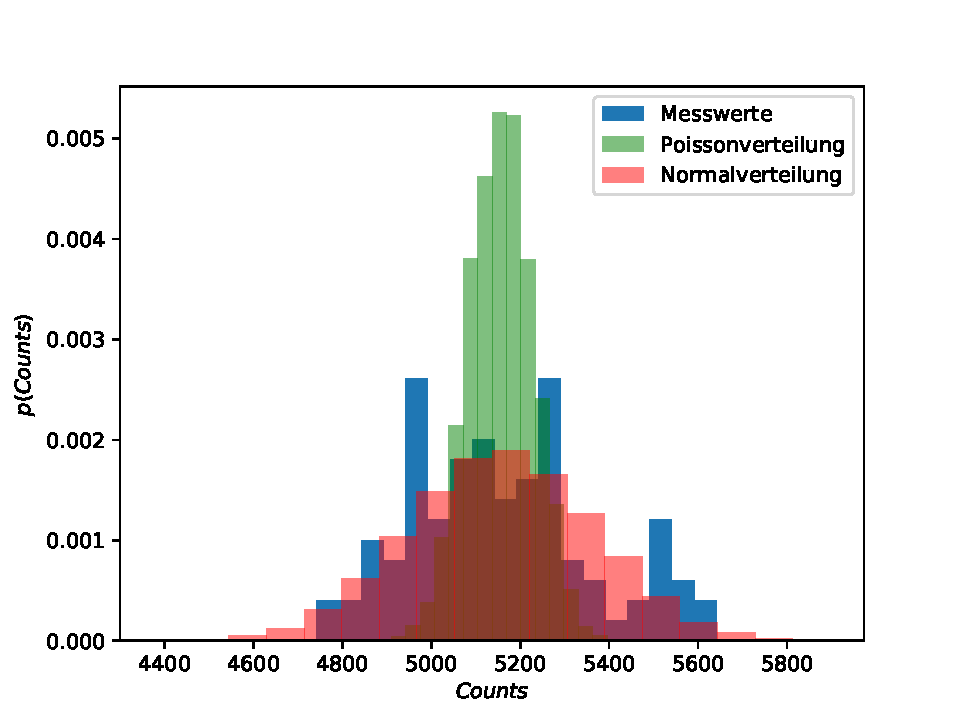
\includegraphics[scale=0.8]{Statistik.pdf}
  \caption{Messwerte mit einer Poisson- und einer Normalverteilung.}
  \label{abb:4}
\end{figure}

\section{Diskussion}
In Tabelle \ref{tab:4} sind die mittleren Reichweite und deren Energien im Vergleich aufgelistet. Zu erkennen sind kleine Abweichungen untereineander,
da aber kein Literaturwert vorliegt, kann keine Aussage über dessen Richtigkeit getroffen werden.
\begin{table}
  \centering
  \caption{Zusammenfassung der Ergebnisse.}
  \label{tab:4}
  \begin{tabular}{c c c}
    \toprule
    & $x_0=\SI{20}{\milli\meter}$ &  $x_0=\SI{25}{\milli\meter}$ \\
    \midrule
    mittlere Reichweite & \SI{15,3}{\milli\meter} & \SI{17,3}{\milli\meter} \\
    Energie der mittleren Reichweite & \SI{2,899}{\mega\eV} & \SI{3,146}{\mega\eV} \\
    \bottomrule
  \end{tabular}
\end{table}

Die erstellte Statistik in Abbildung \ref{abb:4} zeigt die gemessene Verteilung im Vergleich zu einer Poissonverteilung und einer Normalverteilung.
Zu erkennem ist, dass die gemessenen Werte eher einer Normalverteilung entsprechen, dies kann an der geringen Anzahl an Messungen liegen, da diese
Verteilung eigentlich einer Poissonverteilung entsprechen sollte. Außerdem kann der Statistik entnommen werden, dass die Wahrscheinlichkeiten um
den Erwartungswert über der Normalverteilung liegen und sich der Poissonverteilung nähern.

\nocite{*}
\printbibliography
